\section{Poisson solver}
\label{sec:poisson}
\renewcommand{\thesubsection}{\thesection.\arabic{subsection}}
In this section of the lab report, we will dicuss a prallel implementation of the Poisson solver. The Poisson solver is a numerical method used to solve the Poisson equation, which is a partial differential equation that is useful in many areas of physics. \\
\textbf{Note:} For local testing and development I'll run the code with \texttt{mpirun} instead of the \texttt{srun} command on the cluster. \\

\subsection{Building a parallel Poisson solver}
For the first part of the exercise we follow the steps lined out in the assignment sheet. I'll comment on the steps 1 through 10 and related questions bellow. The finished implementation can be found in the appendix for this section. \\
\begin{enumerate}
    \item \textbf{Step:} After adding MPI\_Init and MPI\_Finalize, we can run the program with multiple processes. We can see that the program runs with 4 processes in \autoref{fig:poisson_step1} via the quadrupeled output.
    \begin{figure}[H]
        \centering
        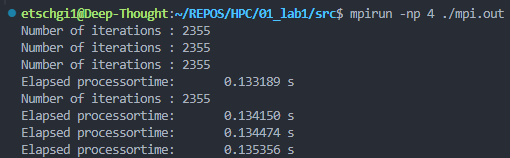
\includegraphics[width=0.5\textwidth]{../fig/lab1/step1.png}
        \caption{MPI\_Poisson after Step 1 - Running with 4 processes}
        \label{fig:poisson_step1}
    \end{figure}
    \item \textbf{Step:} To see which process is doing what, I included the rank of the process for the print statements as shown in \autoref{fig:poisson_step2}.
    \begin{figure}[H]
        \centering
        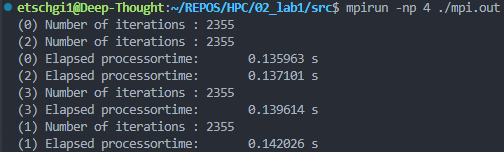
\includegraphics[width=0.5\textwidth]{../fig/lab1/step2.png}
        \caption{MPI\_Poisson after Step 2 - Running with 4 processes}
        \label{fig:poisson_step2}
    \end{figure}
    \item \textbf{Step:} Next we define \texttt{wtime} as a global double and replace the four utility timing functions with the ones given on Brightspace. A quick verification as shown in \autoref{fig:poisson_step3} shows that the program still runs as expected.
    \begin{figure}[H]
        \centering
        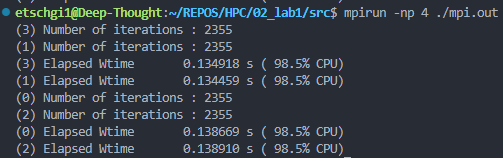
\includegraphics[width=0.5\textwidth]{../fig/lab1/step3.png}
        \caption{MPI\_Poisson after Step 3 - Running with 4 processes}
        \label{fig:poisson_step3}
    \end{figure}
    \item \textbf{Step:} Next we check if two processes indeed give the same output. Both need 2355 iterations to converge and the \texttt{diff} command returned no output, which means that the files content is identical. 
    \item \textbf{Step:} Now only the process with rank 0 will read data from files and subsequently broadcast it to the others. Testing this again with 2 processes, we see an empty diff of the output files and the same number of iterations needed to converge.
    \item \textbf{Step:} We create a cartesian grid of processes using \texttt{MPI\_Cart\_create} and use \texttt{MPI\_Cart\_shift} to find the neighbors of each process. We can see that the neighbors are correctly identified in \autoref{fig:poisson_step6}. 
    \begin{figure}[H]
        \centering
        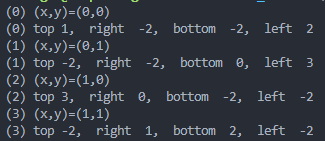
\includegraphics[width=0.5\textwidth]{../fig/lab1/step6.png}
        \caption{MPI\_Poisson after Step 6 - Running with 4 processes on a 2x2 grid}
        \label{fig:poisson_step6}
    \end{figure}
    When there is no neighbor in a certain direction, -2 (or \texttt{MPI\_PROC\_NULL}) is returned. 
    \item \textbf{Step:} We overhaul the setup to get a proper local grid for each process. Furthermore, we only save the relevant source fields in the local grid for each process. \\
    \Shining{With for instance 3 processes you should see that 1 or 2 processes do not do any 
    iteration. Do you understand why?}\\
    If we have a look at the input file we see that there are only 3 source fields in the grid. This means that the process that does not have a source field in its local grid will not do any iterations (or only 1). Therefore, if we have 3 processes and the distribution of source fields as given in the input file only 1 process will do iterations if processes are ordered in x-direction and 2 if ordered in y-direction. From this we can conclude that indeed all processes have different local grids and perform different calculations. 
    \begin{figure}[H]
        \centering
        \begin{minipage}{0.48\textwidth}
            \centering
            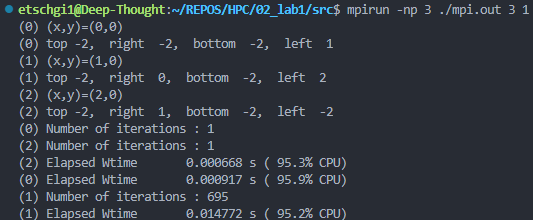
\includegraphics[width=\linewidth]{../fig/lab1/step7a.png}
        \end{minipage}%
        \hspace{0.02\textwidth}
        \begin{minipage}{0.48\textwidth}
            \centering
            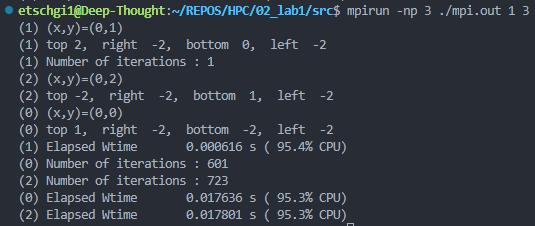
\includegraphics[width=\linewidth]{../fig/lab1/step7b.png}
        \end{minipage}
        \caption{MPI\_Poisson after Step 7 - Running with 3 processes on a 3x1 (left) vs. 1x3 (right) grid\\For the 3x1 grid, only rank 1 does iterations ($> 1$), for the 1x3 grid, ranks 0 and 2 do iterations ($> 1$).}
        \label{fig:poisson_step7}
    \end{figure}
    \item \textbf{Step:} After defining and commiting two special datatypes for vertical and horizontal communication, we setup the communication logic to exchange the boundary values between the processes. We call our \texttt{Exchange\_Borders} function after each iteration (for both red / black grid points). Now we face the problem in which some processes may stop instantly (no source in their local grid). They will not supply any data to their neighbors, which will cause the program to hang. We shall fix this in the next step.
    \item \textbf{Step:} Finally we need to implement the logic to check for convergence (in a global sense). We do this by using a \texttt{MPI\_Allreduce} call with the \texttt{MPI\_MAX} operation. This way we aggregate all deltas and choose the biggest one for the global delta which we use in the while-loop-condition to check for convergence. We can see that the program now runs as expected in \autoref{fig:poisson_step9}.
    \begin{figure}[H]
        \centering
        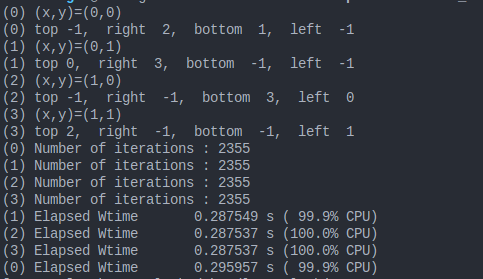
\includegraphics[width=0.5\textwidth]{../fig/lab1/step9.png}
        \caption{MPI\_Poisson after Step 9 - Running with 4 processes on a 2x2 grid}
        \label{fig:poisson_step9}
    \end{figure}
    Note that this run in \autoref{fig:poisson_step9} was done with another pc and another MPI implementation. Therefore, we see $-1$ for cells without a neighbor! However, other than that cosmetic difference it has no impact on the programm. 
    \item \textbf{Step:} Now we only have to fix two remaining things. First we have to make sure that each process uses the right global coordinates for the output file in the end. Therefore, we change the function a bit to include the specific x-/y-offset for each processor. The second thing is the potential problem, that different processors might start with different (red/black) parities. In order to accomplish a global parity we simply have to change the calculation in the if in \texttt{Do\_Step} from 
    \begin{lstlisting}[language=c, lastline=1]
        if ((x + y) % 2 == parity && source[x][y] != 1)
    \end{lstlisting}
    to
    \begin{lstlisting}[language=c, lastline=1]
        if ((x + offset[X_DIR] + y + offset[Y_DIR]) % 2 == parity && source[x][y] != 1)
    \end{lstlisting}
    this guarantees that during a given iteration all processors are using the same parity. 
\end{enumerate}
This just leaves one question open: Are the results acutally the same?\\
Checking the output files of the MPI-implementation with the sequential reference indeed shows identical numerical values for the calculated points. Furthermore, the needed iterationcount is also identical which isn't a big surprise, given that the two programms perform the exact same calculation steps. 

\subsection{Exercises, modifications, and performance aspects}
For this subsection we'll define the following shorthand notation: \\

\begin{table}[h!]
    \centering
    \begin{tabular}{|l|l|}
        \hline
        $n$:  &the number of iterations\\\hline
        $g$:  &gridsize\\\hline
        $t$:  &time needed in seconds\\\hline
        $pt$: & processor topology in form $pxy$, where:\\
        $p$:  &number of processors used\\
        $x$:  &number of processors in x-direction\\
        $y$:  &number of processors in y-direction\\\hline
       \end{tabular}
    \caption{Notation for this section}
\end{table}
$pt = 414$ means 4 processors in a $1\times 4$ topology. \\

\textbf{Note on different Versions:}\\
For the following exercises the implementation will be slightly adapted to measure different performance aspects. To facilitate this, we will use defines to switch between different versions of the code at compile time. The final version of the poissonsolver can be found in the appendix for this section.

\subsubsection{Over-relaxation (SOR)}
We start of by rewriting the \texttt{Do\_Step} routine to facilitate SOR updates. Furthermore, we need $h^2$, the grid spacing (which is 1 in our case) and the relaxation parameter $\omega$ to calculate the updated values. A quick test shows a speedup of roughly a factor of 10. More systematic tests will be done in the next section.
\subsubsection{Optimal $\omega$ for 4 proc. on a 4x1 grid}
With the power of a little python scripting we can easily test different values for $\omega$ and plot the results as seen in \autoref{fig:best_omega_122}. 

\begin{figure}[H]
    \centering
    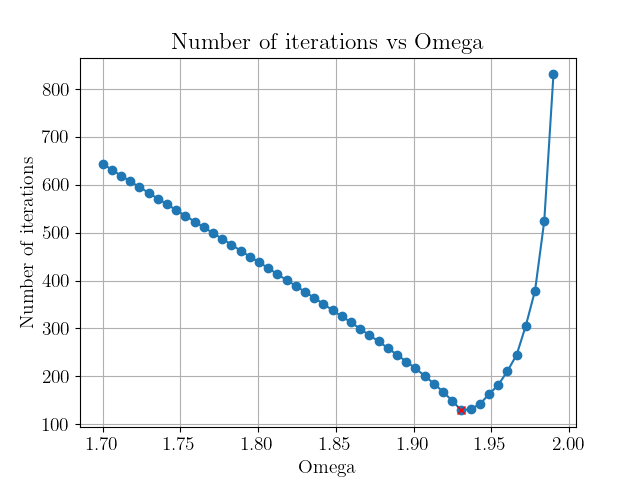
\includegraphics[width=0.7\textwidth]{../fig/lab1/best_omega_122.png}
    \caption{\Shining{Optimal $\omega$ for 4 processors on a 4x1 grid}}
    \label{fig:best_omega_122}
\end{figure}
We find that the optimal $\omega$ is at about $1.93$ for this setup with only 129 iterations. This constitutes a speedup of about 1825\% compared to the sequential implementation. \\

\textbf{N.B.:} If not stated otherwise, we will use $\omega = 1.93$ for the following exercises. 

\subsubsection{Scaling behavior with larger grids}
\label{subsec:scaling}
This investigation is carried out twice: Once with a $4\times 1$ topology (as in the previous section) and once with a $2\times 2$ topology. We use grid sizes of $10\times 10$, $25\times 25$, $50\times 50$, $100\times 100$, $200\times 200$, $400\times 400$, $800\times 800$ and $1600\times 1600$ and set $\omega = 1.95$ for all runs. The results are shown in \autoref{fig:scaling_123}.

\begin{figure}[H]
    \centering
    \begin{minipage}{0.48\textwidth}
        \centering
        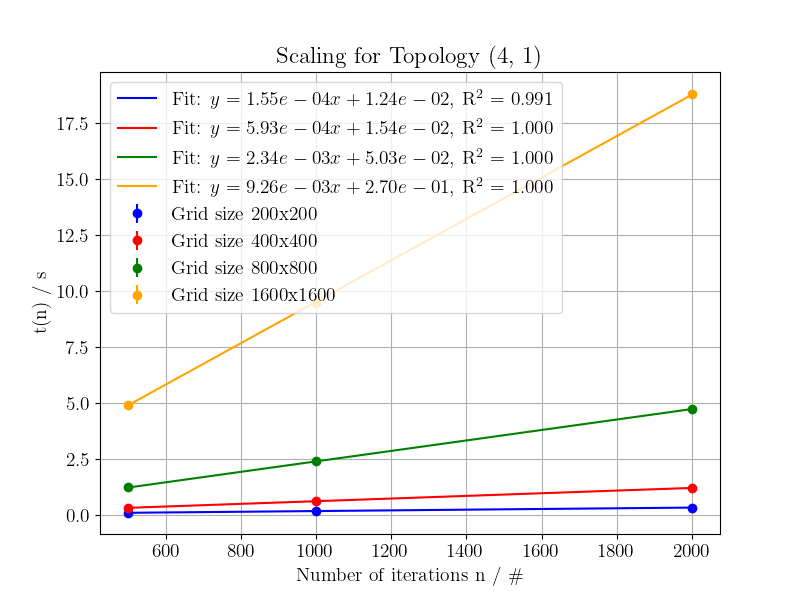
\includegraphics[width=\linewidth]{../fig/lab1/scaling_topology_4x1.png}
    \end{minipage}%
    \hspace{0.02\textwidth}
    \begin{minipage}{0.48\textwidth}
        \centering
        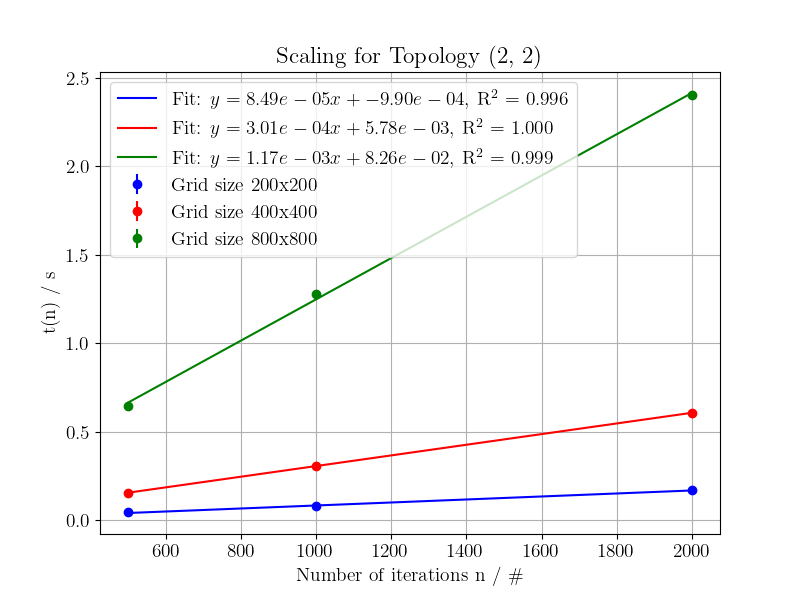
\includegraphics[width=\linewidth]{../fig/lab1/scaling_topology_2x2.png}
    \end{minipage}
    \caption{Scaling behavior of the Poisson solver with different grid sizes and processor topologies}
    \label{fig:scaling_123}
\end{figure}
As seen by the high $R^2$ values in the plots, the scaling behavior is very close to linear. 
We obtain the following scaling factors for the different grid sizes and topologies from the linear fits:
\begin{table}[H]
    \centering
    \begin{tabular}{|c|c|c|}
        \hline
        Topology & $\alpha$ & $\beta$ \\\hline
        $4\times 1$ & $1.35+10^{-1}$ & $7.11+10^{-6}$ \\\hline
        $2\times 2$ & $1.06+10^{-1}$ & $6.17+10^{-6}$ \\\hline
    \end{tabular}
    \caption{Scaling factors for different processor topologies for the Poisson solver\\Using: $t(n) = \alpha + \beta \cdot n$ as a model}
\end{table}
\Shining{What can you conclude from the scaling behavior?}\\
We see that the scaling behavior is very close to linear for both topologies. This means that the parallel implementation scales as expected with the number of grid points.\\
If we compare the scaling factors ($\beta$) for the two topologies we see that the $2\times 2$ topology scales slightly better than the $4\times 1$ topology. This is not surprising, as the $2\times 2$ topology has a more balanced communication workload balance. In the $2\times 2$ topology every processor has two neighbors, while in the $4\times 1$ topology the processors at the ends only have one neighbor. This is a general trend: A topology which divides the grid into square / square-like parts will scale better than a topology which divides the grid into long and thin parts.\\
In essence: We want to keep the communication between processors as balanced as possible to achieve the best scaling behavior.

\subsubsection{Scaling behavior [Theory - no measurements]}
If I could choose between a $16 \times 1$, $8 \times 2$, $4 \times4$, $2 \times 8$, $1 \times 16$ topology, I would choose the $4 \times 4$ topology. This is because the $4 \times 4$ topology has the most balanced communication workload balance, as detailed in the \Shining{Shining} in \autoref{subsec:scaling}.

\subsubsection{Iterations needed for convergence scaling}
We investigate the number of iterations needed for convergence using the $4 \times 1$ topology square grids with sidelength: $10, 25, 50, 100, 200, 400, 800, 1600$. The results for different \Shining{$\omega$} are shown in \autoref{fig:iterations_125}.

\begin{figure}[H]
    \centering
    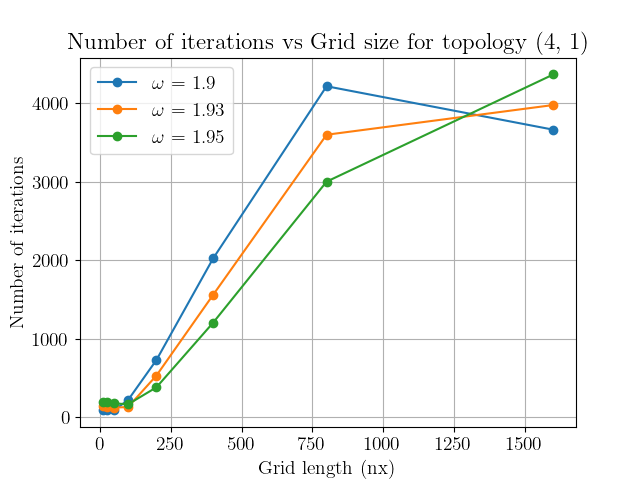
\includegraphics[width=0.7\textwidth]{../fig/lab1/iteration_count_(4, 1)_125.png}
    \caption{Iterations needed for convergence with different grid side lengths}
    \label{fig:iterations_125}
\end{figure}
We can clearly see that the number of iterations till convergence increases with the problem size. At first, I expected linear growth proportional to the number of gridpoints. However, it turns out that the number of iterations actually grow slower and in a square root like fashion. This can be seen by the linear behavior in the plot of grid-side length against iterations. 

\Shining{Why is the number of iterations needed for convergence $\propto \sqrt{g}$?}\\
Our poisson problem is a discretized system in 2D space. The condition number of the matrix we have to solve is proportional to the number of gridpoints in our system. SOR uses the spectral properties of the matrix to solve in a way such that the dominant error mode takes time proportional to the diameter of the domain to converge. This means it is proportional to $\sqrt{g} = \sqrt{n_x \cdot n_y}$.\\

\Shining{Why does omega with the best performance change with the grid size?}\\
As can be seen in \autoref{fig:iterations_125} $\omega = 1.9$ beats the other two values for very small and the largest gridsize. For different gridsizes we get differnetly sized matrices we have to solve. SOR overrelaxes high-frequency errors and underrelaxes low-frequency errors (the later for stability). The optimal $\omega$ is therefore dependent on the gridsize and the error modes present in the system. In our current example, it might be that $\omega = 1.9$ is a good compromise for the grid sizes we are looking at.

\subsubsection{Error as a function of the iteration number}
With the same $4 \times 1$ topology and grid sizes of $800 \times 800$ the error for $15000$ iterations is tracked using $\omega = 1.93$. The results are shown in \autoref{fig:error_126}.
\begin{figure}[H]
    \centering
    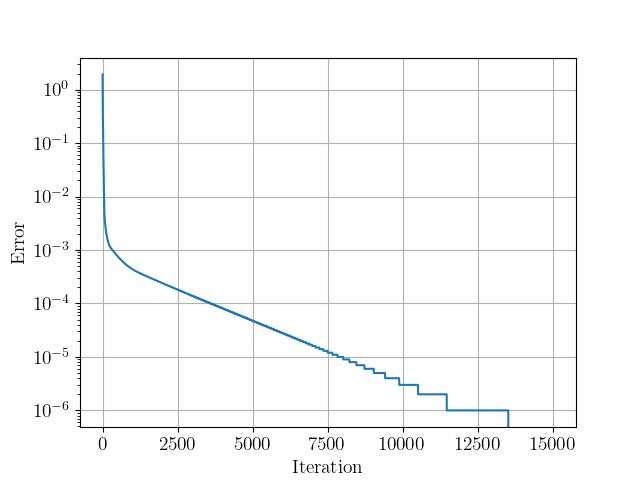
\includegraphics[width=0.7\textwidth]{../fig/lab1/errors_126.png}
    \caption{Error as a function of the iteration number}
    \label{fig:error_126}
\end{figure}
At first the error decreases rapidly in the first few iterations to about $10^{-3}$ (logarithmic scale!). After that the error decreases more slowly until it is below floating point precision. \Shining{Note:} All calculations are done using double precision floating point numbers and only the error recording was done using single precision which leaves the step-like artifacts in the plot. 

\subsubsection{\Shining{Optional} - Gain performance by reducing \texttt{MPI\_Allreduce} calls}
The last subsection showed us that the error reduces monotonically. We might be able to save some time by leaving out some checks and maybe check the global error every 10th or 100th iteration only.\\ First, we should benchmark if it is at all wise to optimize here, by measuring how long the \texttt{MPI\_Allreduce} call takes. We can do this by measuring the time needed for the \texttt{MPI\_Allreduce} call in the \texttt{Do\_Step} function and summing up to get the total time spent in \texttt{MPI\_Allreduce} calls.\\
We again solve with a $4 \times 1$ topology, $\omega = 1.93$ and a $800 \times 800$ grid: It takes roughly $20$ seconds of which the processors spend around 1 - 2 seconds in the \texttt{MPI\_Allreduce} call. This is a significant amount of time ($(7.0 \pm 0.4)$\%). This means we would save some time by reducing the number of \texttt{MPI\_Allreduce} calls and calculating 9 (0.25\% of total) more iterations wouldn't hurt us too bad because it takes 3601 to converge!\\
We run the program three times with \texttt{MPI\_Allreduce} calls every 1, 10 and 100 iterations and get the speedups in \texttt{MPI\_Allreduce} calls as shown in \autoref{tab:allreduce_speedup}.
\begin{table}[H]
    \centering
    \begin{tabular}{|c|c|c|}
        \hline
        Iterations & \texttt{MPI\_Allreduce} - speedup (factor) & calculated overall speedup (\%)\\\hline
        1  & 1.00 & 0\\\hline
        10 & $6.0 \pm 2.0$ & $ 5.9 \pm 0.5$\\\hline
        100& $62 \pm 6$    & $ 6.9 \pm 0.4$\\\hline
    \end{tabular}
    \caption{Speedup in \texttt{MPI\_Allreduce} calls for different iteration counts and calculated overall speedup (\%)}
    \label{tab:allreduce_speedup}
\end{table}
As can be clearly seen from the table we can gain around 6 \% using \texttt{MPI\_Allreduce} calls every 10 iterations and around 7 \% using \texttt{MPI\_Allreduce} calls every 100 iterations. This is a significant speedup for a very small change in the code.\\
\textbf{Note:} The speedup is calculated to account for fluctuations in the runtime of the program, due to other processes running on the same machine / cluster. 

\subsubsection{Reduce border communication}
Another way to reduce communication overhead is to reduce the number of border exchanges. To investigate if this yields a speedup  we run the program on a $4 \times 1$ topology, $\omega = 1.93$ and different grid sizes and track the iterations and time as seen in \autoref{fig:border_speedup}.

\begin{figure}[H]
    \centering
    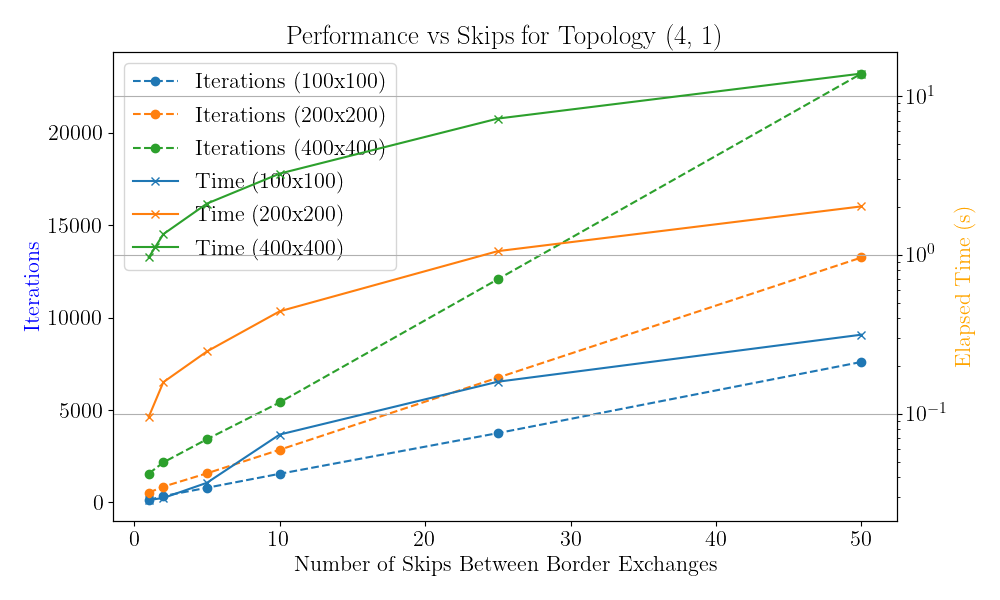
\includegraphics[width=0.7\textwidth]{../fig/lab1/skips_topology_4x1.png}
    \caption{Speedup by reducing border exchanges}
    \label{fig:border_speedup}
\end{figure}

Running the with different numbers of skipped border exchanges naturally slows down convergence, meaning we need more iterations to reach the same error. For all tested grid sizes the initial SOR version without skipping border exchanges has the fewest iterations needed to convergence and also the fastes runtime. \\

\Shining{What can you conclude from the results?}\\
We can conclude that reducing the number of border exchanges does not yield a speedup. The reason for this is that we have to calculate more iterations to converge to the solution which outweighs the gains from reduced communication overhead. Interestingly, for the $100 \times 100$ grid there exists a local minimum in time at 4 skipped border exchanges compared to 3 skipped. This is likely due to our source field distribution and thus specific to our problem.

\subsubsection{Optimize \texttt{Do\_Step} loop}

In \texttt{Do\_Step} we iterate over the whole grid but only update one of the two parities at a time. This means we can split the loop into two loops, one for each parity. We start out with something like this:
\begin{lstlisting}[language=c]
    for (x = 1; x < dim[X_DIR] - 1; x++){
        for (y = 1; y < dim[Y_DIR] - 1; y++){
            if ((x + offset[X_DIR] + y + offset[Y_DIR]) % 2 == parity && source[x][y] != 1){
                ...
\end{lstlisting}
and we change it to:
\begin{lstlisting}[language=c]
    int start_y;
    for (x = 1; x < dim[X_DIR] - 1; x++){
        start_y = ((1 + x + offset[X_DIR] + offset[Y_DIR]) % 2 == parity) ? 1 : 2;
        for (y = start_y; y < dim[Y_DIR] - 1; y += 2){
            if (source[x][y] != 1){
                ...
\end{lstlisting}
The basic idea is to avoid y-coordinates which are not in the parity we are currently updating. 
We measure 10 runs for a $800 \times 800$ grid and a $4 \times 1$ topology with $\omega = 1.93$ and get the following times: 
\[t_{\text{no\_improvements}} = \SI{5.59(5)}{\second}\hspace{1cm}\text{and}\hspace{1cm}t_{\text{loop\_improvements}} = \SI{4.64(7)}{\second}\]
So we get a minimal speedup of about 17\% by optimizing the loop which is a enormous speedup for such a small change.

\Shining{Why does this make such a difference}\\
The reason for this is that we avoid unnecessary looping and if statements. This means that we have less overhead in the loop and can therefore calculate faster by skipping the unnecessary loop entries. 

\subsubsection{\Shining{Optional} - Time spent within \texttt{Exchange\_Borders}}
We can measure the time spent in \texttt{Exchange\_Borders} by adding a timer to the function. We run the program with $\omega = 1.93$ and different topologies and grid sizes and get the results shown in \autoref{fig:exchange_time}.
\begin{figure}[H]
    \centering
    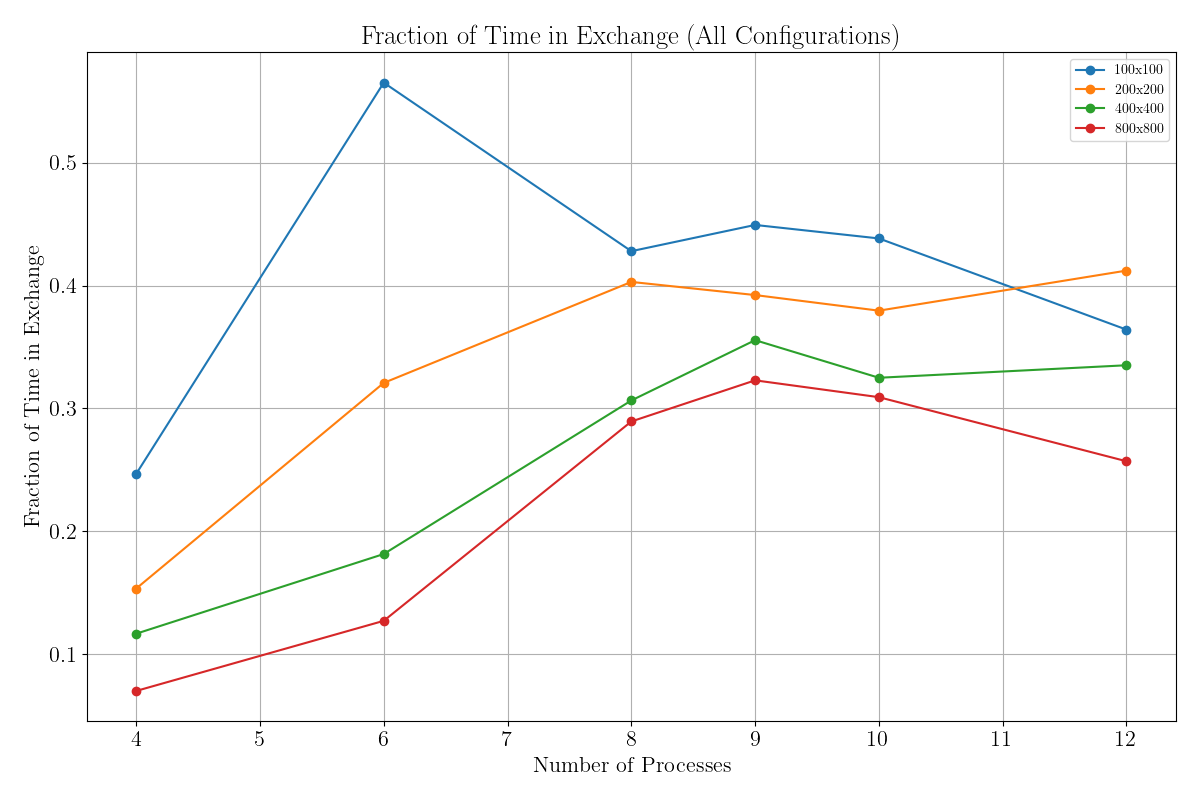
\includegraphics[width=0.7\textwidth]{../fig/lab1/fraction_exchange_comparison_connected.png}
    \caption{Fraction of total time spent in \texttt{Exchange\_Borders}}
    \label{fig:exchange_time}
\end{figure}
As we can clearly see, the time spent in \texttt{Exchange\_Borders} is initially smaller and grows with processor count. The curves are generally shifted downward for larger gridssizes. \\

\Shining{Interpretation:}\\
One would expect larger grid sizes to be more computationally expensive and we have already established that iterations take longer the bigger the grid. Communication obviously also takes longer for a larger grid because we have more data to sent. However, the circumference of a square grows linearly, while the area grows quadratically. The quadratic growth of the area is the reason for the downward shift in the curves for larger grid sizes because the communication overhead grows slower than the computational overhead for larger grids.\\

\Shining{When is the time spent in \texttt{Exchange\_Borders} significant / comparable to computation?}\\
As can be seen in \autoref{fig:exchange_time} the time spent in \texttt{Exchange\_Borders} is significant for all grid sizes from the start (between 5 and 25\%). Thereafter it grows to around 30\% to 45\% for 9 processors. This means that the time spent in \texttt{Exchange\_Borders} is significant for all grid sizes and processor counts, but especially as the processor count grows.

\subsubsection{Latency and bandwith in \texttt{Exchange\_Borders}}
We use the configurations from \autoref{subsec:scaling}: $4 \times 1$, $2 \times 2$ and \Shining{$3 \times 3$} topologies with grid sizes of $200 \times 200$, $400 \times 400$ and $800 \times 800$ and $\omega = 1.95$. We obtain the results in \autoref{tab:latency_bandwith}.
\begin{table}[H]
    \centering
    \caption{Metrics for \texttt{Exchange\_Borders} latency and bandwith}
    \label{tab:latency_bandwith}
    \begin{tabular}{|l|l|S[table-format=3(3)]|S[table-format=1.1]|S[table-format=9]|S[table-format=9]|}
    \hline
    Topology & Grid Size & {Latency (ms)} & {Latency (\%)} & {Bandwidth (\si{\byte\per\second})} & {Total Data (\si{\byte})} \\\hline
    4x1 & 200x200 & 370(44) & 6.6 & 447314206 & 135548032 \\\hline
    4x1 & 400x400 & 328(39) & 6.0 & 511267773 & 135548032 \\\hline
    4x1 & 800x800 & 401(38) & 7.1 & 390446955 & 135548032 \\\hline
    2x2 & 200x200 & 346(83) & 6.2 & 426689734 & 108546432 \\\hline
    2x2 & 400x400 & 281(74) & 5.2 & 576865986 & 108546432 \\\hline
    2x2 & 800x800 & 288(71) & 5.3 & 558562482 & 108546432 \\\hline
    3x3 & 200x200 & 1054(204) & 25.2 & 78386044 & 72364288 \\\hline
    3x3 & 400x400 & 1147(229) & 27.6 & 81623075 & 72364288 \\\hline
    3x3 & 800x800 & 1082(148) & 26.7 & 60819112 & 72499296 \\\hline
    \end{tabular}
\end{table}
\Shining{Interpretation:}\\
As can be seen the latency is more or less comparable between the $4 \times 1$ and $2 \times 2$ topologies. The $3 \times 3$ topology has a significantly higher latency. This is due to the fact that the $3 \times 3$ topology has more neighbors to communicate with. 

\subsubsection{Exchange Border potential improvements}
Indeed we communicate twice as much as we need after each \texttt{Do\_Step} call. We shall analyze this considering the following points: 
\begin{itemize}
    \item address of the first point to exchange: This depends on the parity of the processor. It is simply the first or second point in the grid depending on the parity (leaving out the edge case where the processor only has one data-point).
    \item the number of points to exchange: This normally is the number of points in the grid minus ghost cells divided by two. However, this may change if there is an odd number of points in the grid (then we have to exchange one more or one less point).
    \item the number of points in between grid points that have to be exchanged: The stride of the data will change. Currently we exchange every point for one direction and every \texttt{dim[Y\_DIR]}-th point for the other direction. This can be optimized to exchange every second point in one direction and every second \texttt{dim[Y\_DIR]}-th point in the other direction. 
\end{itemize}

\textbf{Is it worth it?}\\
For smaller gridsizes it is not worth it to optimize the border exchange. The time spent in the border exchange might be significant in relative terms, but the absolute time is still small. For larger gridsizes it might be worth it to optimize the border exchange. As we have seen, this becomes more significant as the processor count and gridsizes grow. For our current problem and similarly sized problems the effort put into optimizing the border exchange is certainly not worth it.